\subsection{Classification of Simultaneously Played Strokes} \label{section:methodCombined}

So far, only single strokes at the same time are analyzed. But usually, when playing a drum set, multiple drums and cymbals are used at the same time. Therefore, this section introduces two approaches to classify simultaneously played strokes. Both approaches are based on the templating method in section \ref{section:shapeComparisonClassification3}, which calculates the distance from a predefined acceptable range. To test these methods, a new test set is created, which contains the most common combinations of two drums, a drum and a cymbal or two cymbals. The following combinations are chosen:

% Liste getester kombis
\begin{itemize}
  \item Bass drum with snare drum
	\item Bass drum with closed hi-hat
	\item Bass drum with opened hi-hat
	\item Snare drum with closed hi-hat
	\item Tom 1 with tom 3
	\item Crash cymbal with ride cymbal
\end{itemize}

\subsubsection{Test set}
\label{section:multipleTestset}
As test set, other test instances are needed, which contain the above chosen stroke combinations. But to gain comparable results, the same recordings as used for the single drum tests are used. To gain simultaneous strokes, the sound of these records is superimposed with the help of MatLab\textsuperscript{\textregistered}. To generate the superimposed strokes, two single stroke records \lstinline{Y1} and \lstinline{Y2} are used and combined with the help of the following method:

\begin{enumerate}
  \item Finding the position \lstinline{o1} of the first onset in \lstinline{Y1} and the position \lstinline{o2} of the first onset in \lstinline{Y2} with the help of the onset detector described in section \ref{section:onsetdetectionmethod}.
	\item Calculating the duration between zero and the onset with the minimum position as \lstinline{beforeOnset} by \lstinline{beforeOnset = min(onset1, onset2)}.
	\item Calculating the duration between to onset with the maximum position and the end of the recording as \lstinline{afterOnset} by \lstinline{afterOnset = min(length(y1)-onset1, length(y2)-onset2)}.
	\item Building the combined audio wave \lstinline{Y} by superimposing the onsets \lstinline{o1} and \lstinline{o2} with \lstinline{y1(o1-beforeOnset+1:o1+afterOnset) + y2(o2-beforeOnset+1:o2+afterOnset)}.
\end{enumerate}

The function is described in figure \ref{fig:superimpose}.

\begin{figure}[htb]
	\centering
	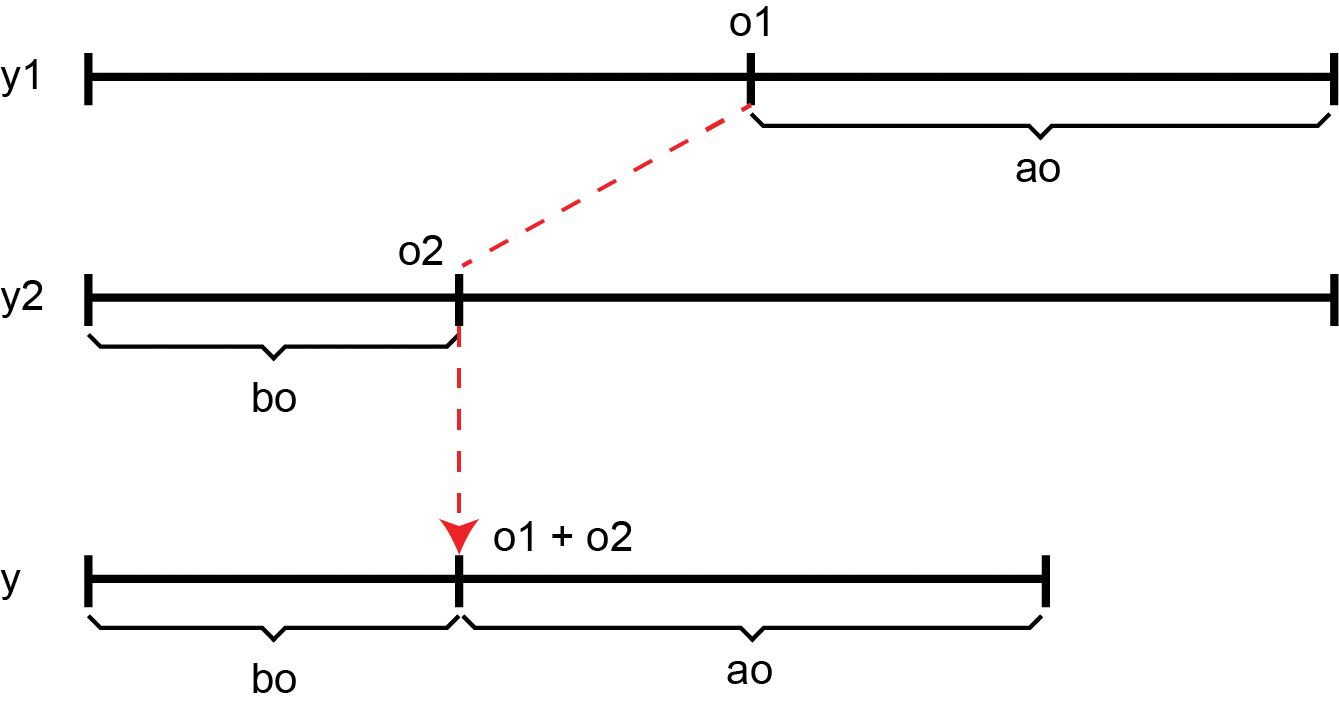
\includegraphics[height=5cm]{images/superimposition.png}
	\caption{Superimposition of two single stroke recordings.}
	\label{fig:superimpose}
\end{figure}

\subsubsection{Classification of Simultaneous Strokes by Subtraction}

The first developed method for classifying multiple drums played at once is based on subtraction of the frequency spectrum. For this method an additional template is created, which contains the mean frequency spectrum of all training instances of a stroke type. It is created in the same manner as the minimum/maximum templates, which is described in section \ref{section:shapeComparisonTemplates}. The only difference is that the mean value is calculated instead of using the quantile function. For the creation of the mean template \lstinline{AMean}, the \lstinline{createTemplates} function, which is displayed in listing \ref{lst:templates}, is extended. The entire function is shown in listing \ref{lst:templates2}.

\begin{lstlisting}[caption={Template creation including mean template.},label={lst:templates2}]
function[AMin,AMax,AMean]=createTemplates(A,n)
	AMin=zeros(length(A(:,1))/n,length(A(1,:)));
	AMax=zeros(length(A(:,1))/n,length(A(1,:)));
	AMean=zeros(length(A(:,1))/n,length(A(1,:)));
	locDrum=0;
	for i=1:n:length(A(:,1))				
		Atmp=A(i:i+n-1,:);
		locDrum=locDrum+1;				
		%% quantile
		AMax(locDrum,:)=quantile(Atmp,0.99);
		AMin(locDrum,:)=quantile(Atmp,0.01);
		%% mean
		AMean(locDrum,:)=mean(Atmp);  
	end
end
\end{lstlisting}

The first step of this method is equal to the method used to classify single drums by using the distance from the acceptable range as described in section \ref{section:shapeComparisonClassification3}. The result of this method is a class label for one of the played drums or cymbals in the tested frame. To get the second drum or cymbal, the subtraction algorithm is added. It subtracts the mean frequency spectrum \lstinline{AMean} of the detected stroke type from the test frames frequency spectrum. The creation of the template \lstinline{AMean} was explained in section \ref{section:shapeComparisonTemplates}. The values are subtracted with a factor of 1.3 to ensure that an already detected drum or cymbal cannot be detected as second drum again. Subsequently, the values smaller than zero are set to zero and the resulting spectrum is normalized again by dividing all its values with the mean of all values. The entire subtraction process is shown by the MatLab\textsuperscript{\textregistered} code in listing \ref{lst:subtraction}. 

\begin{lstlisting}[caption={Subtraction of the mean spectrum of the extracted class label from the frequency spectrum of a frame with two drums played at once.},label={lst:subtraction}]
Atmp2 = Atmp - AMean(idx,:)'.*1.3;
Atmp2(Atmp2<0) = 0;         %set negative values to zero
Atmp2=Atmp2./mean(Atmp2);   %normalize 
\end{lstlisting}

After the subtraction and normalization, the second drum can be detected by running the distance algorithm for single drums, which was also used to classify the first stroke of the record, again.

The results of this method are summarized in a confusion matrix in figure \ref{fig:multiple11}. The matrix shows with which two class labels the particular test records are classified. The input data is placed on the left column, the classification results on the top. The green values show the number of test records for which both strokes are classified with the right class labels. The yellow colored fields display the number of records for which only one of the two strokes is classified correctly. The orange field shows the number of incorrect classified instances for both strokes in a record. 120 different test records are tested. The result shows that about 69.17 \% of the records are classified with two correct class labels. This equals a total of 83 correctly classified test instances. Moreover, 32 instances (~26.67 \%) are classified with one correct and one incorrect class label and five instances (~4.17 \%) are classified with two incorrect class labels.

The best results are gained for the tested combinations of two drums (without a cymbal). These are the combination of bass drum and snare drum, as well as the combination of tom 1 and tom 2. For bass and snare, nine out of ten correctly classified instances are reached for both low and  high powered strokes. One low powered stroke is classified as bass drum with closed hi-hat. One high powered stroke is classified as snare drum with tom 1. For tom 1 with tom 2, nine correctly classified instances are achieved for low powered strokes and ten for high powered ones. The incorrectly classified instance is labeled with tom 3 twice.

Stroke combinations containing the closed hi-hat show high hit-rates if low powered strokes are used. For the combination of snare drum and closed hi-hat, there are nine correctly classified instances with low powered strokes and five for high powered ones. The remaining instances are classified as either two snare drums or as snare drum combined with tom 1. For the combination of the closed hi-hat with the bass drum, all test instances are classified correctly for low powered and five for high powered strokes. The incorrectly classified records are classified as a combination of bass drum and snare drum.

Stroke combinations containing the opened hi-hat, the crash cymbal and the ride cymbal cause a higher error rate than stroke combinations containing only drums or the closed hi-hat. The opened hi-hat is easily confused with the closed hi-hat. Thus, the test records with the opened hi-hat and the bass drum show only three correctly classified instances for low powered strokes. The remaining strokes are classified as bass drum with closed hi-hat. For high powered strokes, there are seven correctly classified instances, one is declared as bass with hi-hat closed, one as two bass drums and one as hi-hat opened with snare drum. The combination of crash and ride cymbal show most misses of all tested instances. For low powered strokes, there are no correctly classified instances.

%% RESULTS
% 120 test records
% 83 green (69,17%)
% 32 yellow (26,67%)
% 5 red (4,17%)
\begin{figure}[htbp]
	\centering
	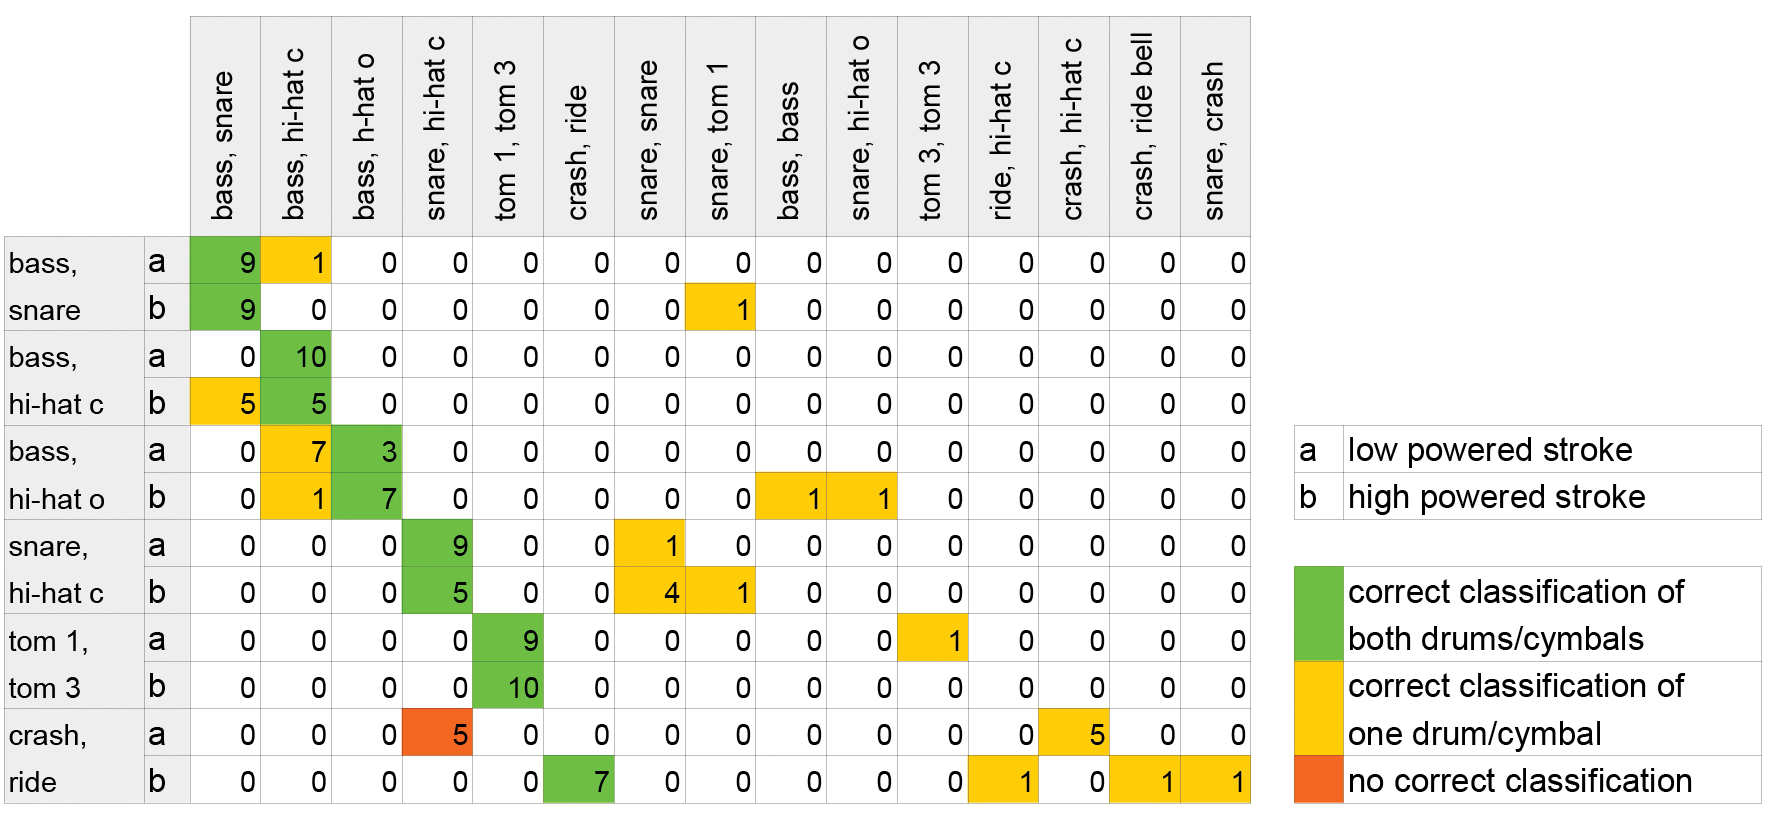
\includegraphics[width=.8\textwidth]{images/classification_matrix/multiple1_test_1.png}
	\caption{Results for the subtraction algorithm tested with recordings containing two strokes at once.}
	\label{fig:multiple11}
\end{figure}

In the preceding step, the fact that also only one drum could be played at a time has not been considered. But with the used method two class labels are assigned to every test record. To avoid that, the algorithm should be able to return null as class label, which means that no drum was played. Therefore, the training set is extended by a record containing noise. If the detected class label for the second drum is noise, only one drum or cymbal is played. The noise is trained in the same way as the different strokes. Since there is no onset, it is set to the 512th sample in the noise audio wave. A drum or cymbal is correctly classified if it is labeled with the tested stroke type and nil or with twice the tested stroke type.

The described function is tested with both, the test set containing simultaneously played strokes and the test set containing single strokes. The results are displayed in figures \ref{fig:multiple12} and \ref{fig:multiple13}. Figure \ref{fig:multiple12} shows the results for the tested single drums. Figure \ref{fig:multiple13} the results for the multiple drum combinations.  

The test set for single drums contains a total of 280 test instances. For 276 instances (98.57 \%) the correct drum type can be detected. But for 146 instances (52.14 \%) of them a second drum or cymbal is detected. Thus, there are only 130 instances (46.43 \%) labeled with two correct class labels. Further on, both  labels  are declared incorrectly for four instances (1.43 \%). 

%% RESULTS
% ges 280
% 130 green (46,43%)
% 146 yellow (52,14%)
% 4 red (1,43%)
\begin{figure}[htbp]
	\centering
	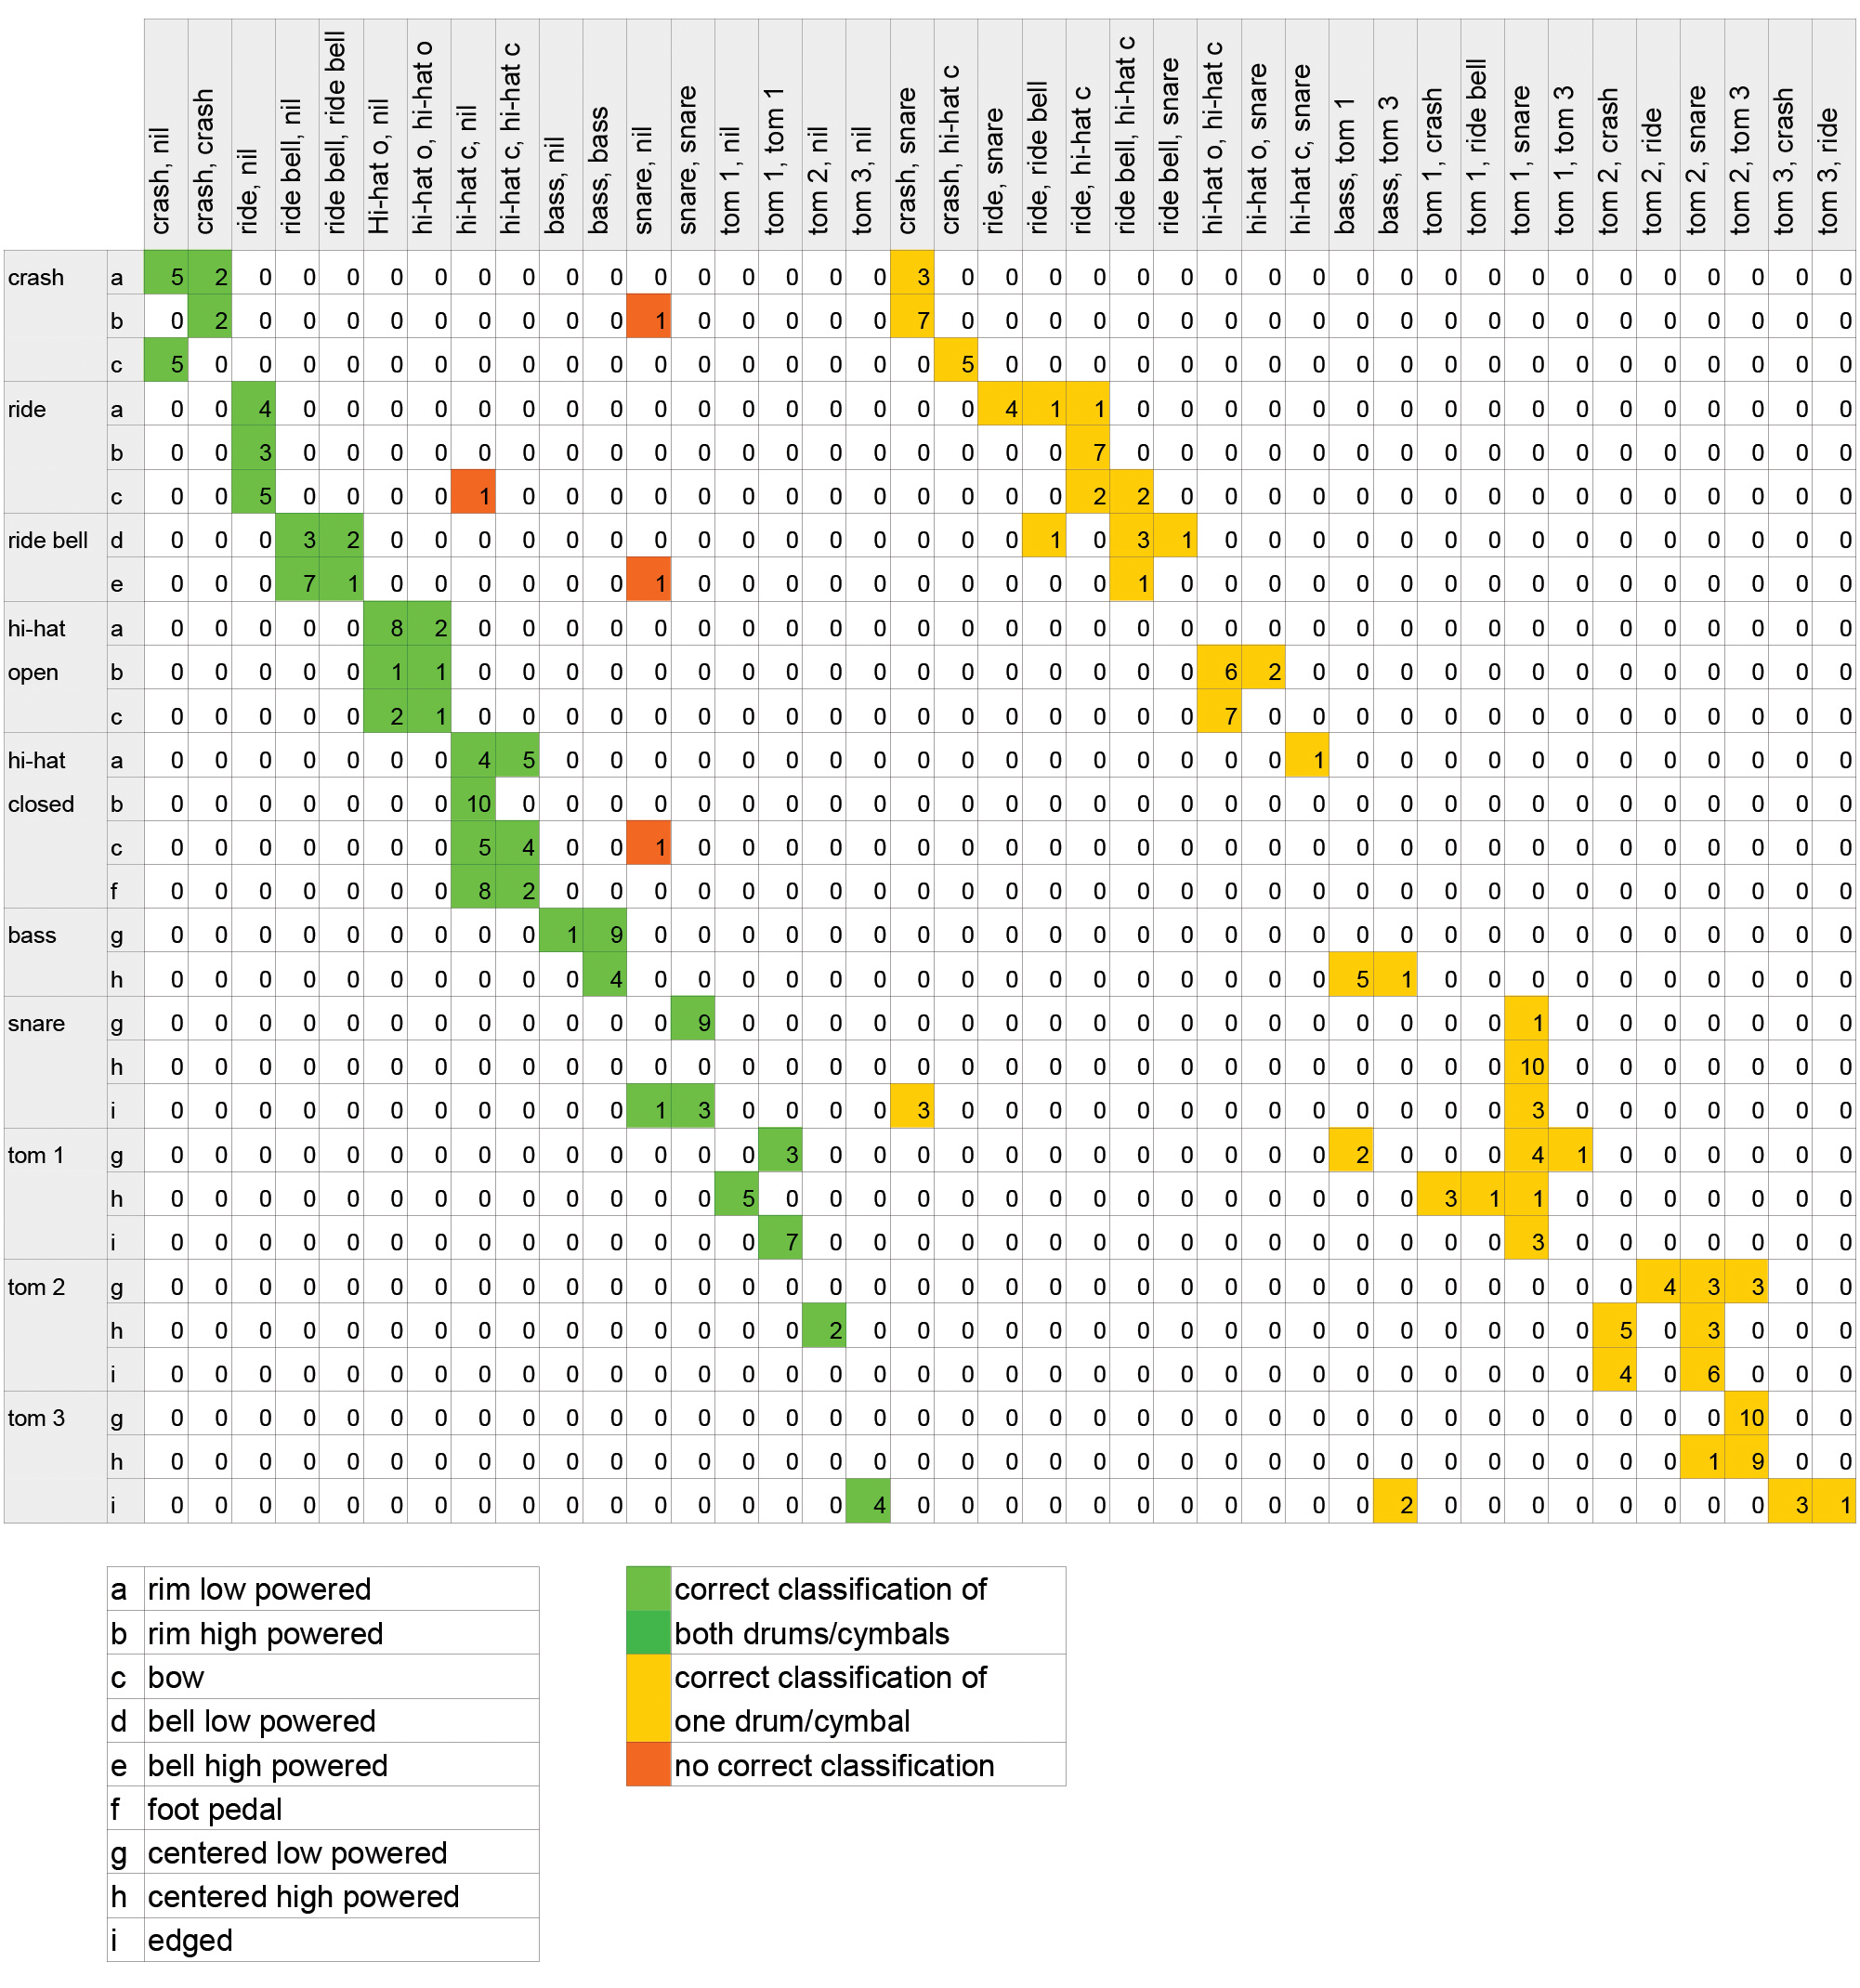
\includegraphics[width=\textwidth]{images/classification_matrix/multiple1_test_2_single.png}
	\caption{Results for the subtraction algorithm including the training with noise tested with recordings containing single strokes.}
	\label{fig:multiple12}
\end{figure}

The results for multiple drums (figure \ref{fig:multiple13}) show 15 \% less correctly classified instances than the results of the method without noise. There are 65 instances (54,17 \%) classified with two correct class labels, 50 instances with one and five instances with no correct class label. Differences are mainly detected in test records that contain the snare drum and the closed hi-hat. Here, the snare drum is detected but the second label is declared as null. Only one record containing a low powered stroke is correctly classified. Furthermore, there are several other test instances for which the second drum is classified as null instead of the correct class label.

%% RESULTS
% ges 120
% 65 green (54,17%)
% 50 yellow (41,67%)
% 5 red (4,17%)
\begin{figure}[htbp]
	\centering
	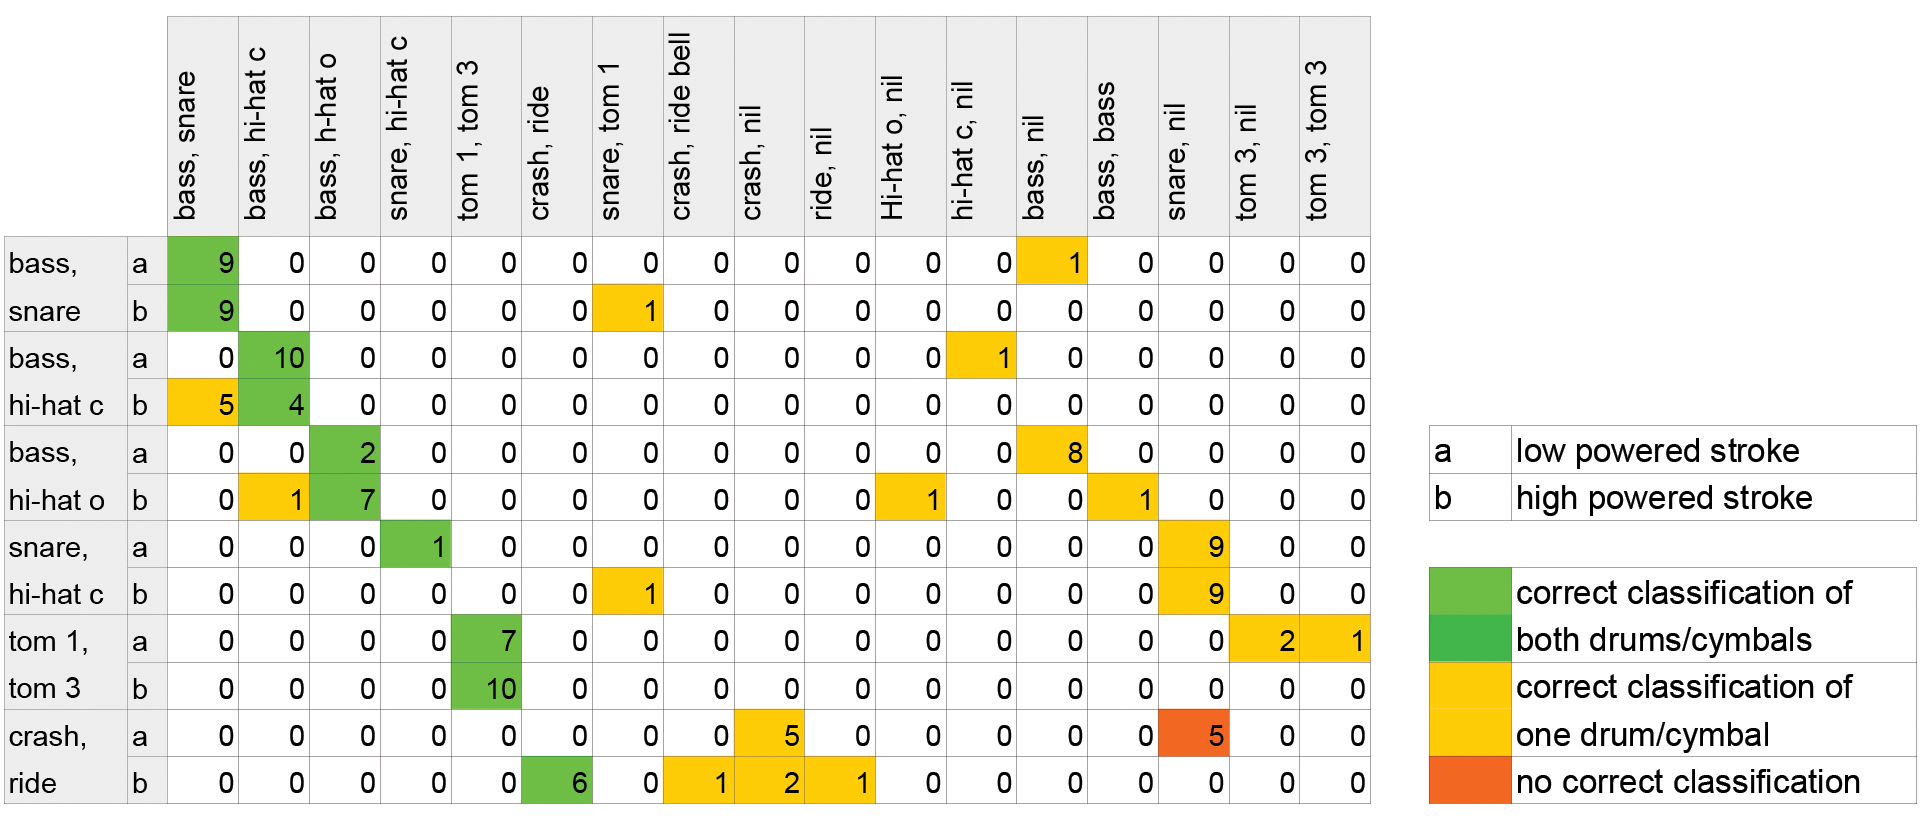
\includegraphics[width=.9\textwidth]{images/classification_matrix/multiple1_test_2_multiple.png}
	\caption{Results for the subtraction algorithm including the training with noise tested with recordings containing two strokes at once.}
	\label{fig:multiple13}
\end{figure}


% explain why there is a problem with noise training
The results show that the training with noise causes classification errors. The reason for these errors can be explained by the noise reduction and normalization. Whereas these steps improve the hit-rate for the classification of only one drum played at once, it leads to errors for the second drum. The classification algorithm subtracts the noise from the spectrum before the first drum is classified. Afterward, the mean spectrum of the stroke classified as first label is also subtracted. Thus, assuming there exists no second stroke in the spectrum, all remaining values should be zero or nearly zero. If the spectrum is normalized after this again, the resulting values are very random and match neither the noise nor any of the trained stroke types. Thus, the algorithm chooses the most similar training record as label which can easily be another one than the noise record. The same problem appears for the training of the noise record. Here, the noise is also subtracted and the spectrum is normalized after this. Thus, the noise training records also result in random spectra that can be similar to one of the trained drums or cymbals. 

Hence, a second algorithm for the classification of two drums played at once, which does not use the noise as training instance, is developed in the following section.

\subsubsection{Classification of Simultaneous Strokes by Extension of the Training Set}

The second developed method to classify several drums played at once is based on the additional training of the possible combinations of drums. Thereby, the stroke combinations are trained by superimposing the appropriate single strokes as explained in section \ref{section:multipleTestset}. By the use of this method it is avoided that the user has to train the system with all possible combinations of drums and cymbals. After the training, the classification algorithm based on the distance from the acceptable area described in section \ref{section:shapeComparisonClassification3} is used.

To test the algorithm, firstly the test set with single drums and secondly the test set with multiple strokes played at once is used. The results for the single drums are displayed in figure \ref{fig:multiple21}. It is observed that none of the test records is classified with two class labels. The results remain exactly the same as for the algorithm tested without the training of multiple drums. These results were described in section \ref{section:shapeComparisonClassification3}.

%% RESULTS
\begin{figure}[htbp]
	\centering
	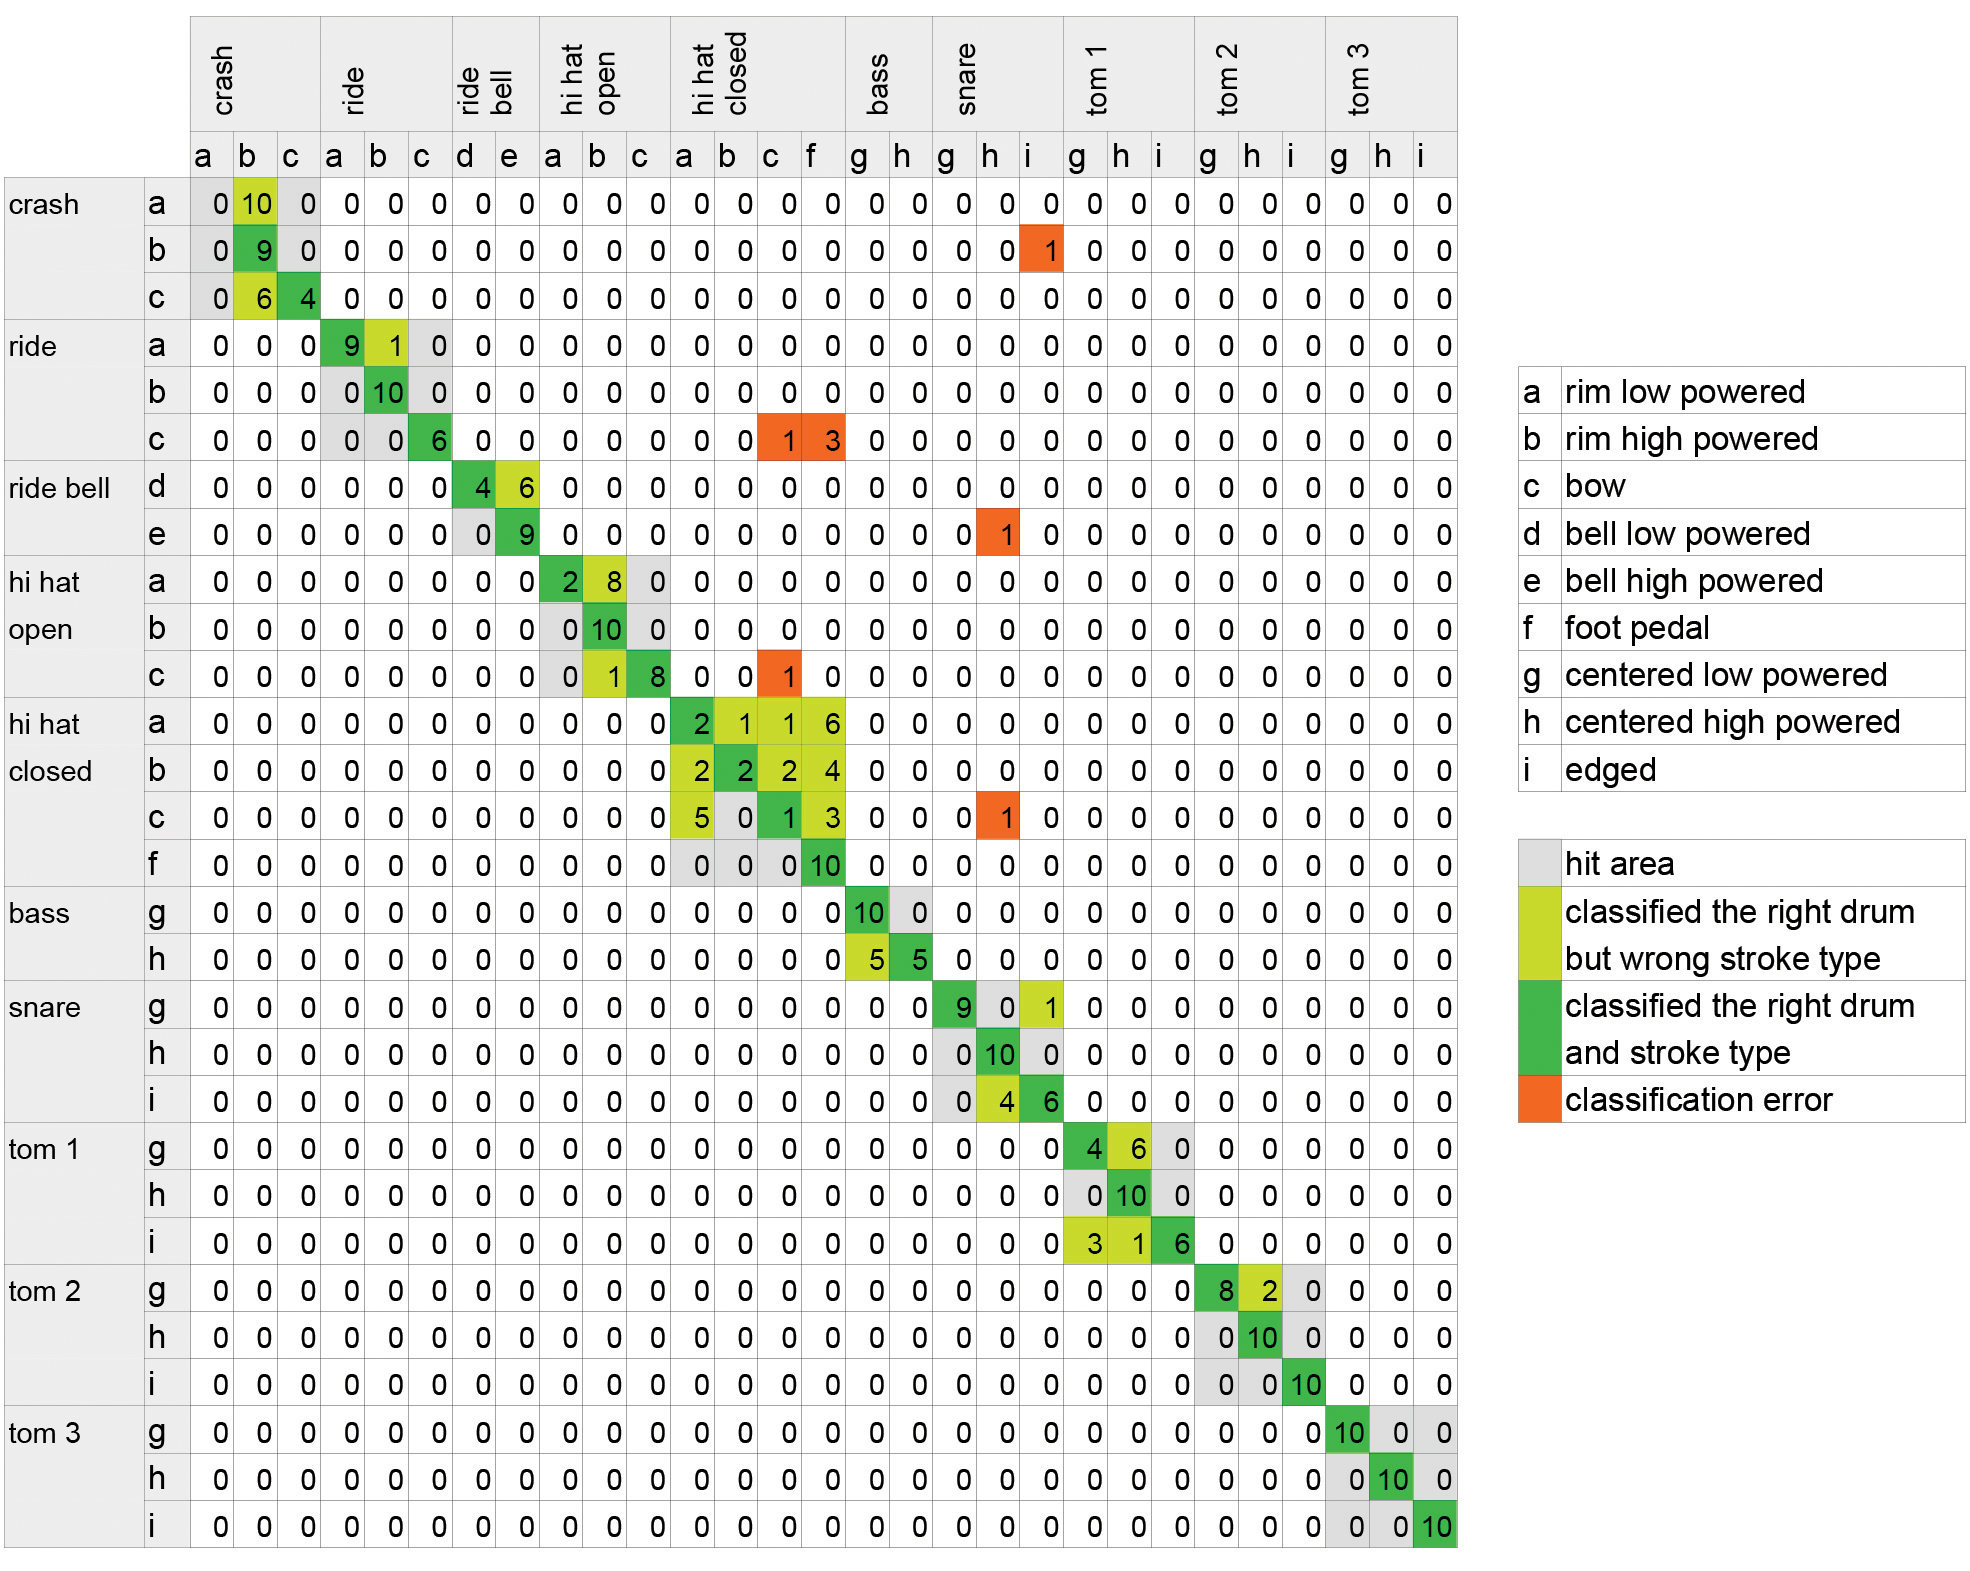
\includegraphics[width=\textwidth]{images/classification_matrix/multiple2_test_single.png}
	\caption{Results for the extended training algorithm tested with recordings containing single strokes.}
	\label{fig:multiple21}
\end{figure}


Figure \ref{fig:multiple22} summarizes the results for the test set containing the recordings with two drums played at once. The test set contains 120 instances and twelve different stroke types. There are ten instances for each stroke type.

As for the tests with single drums, the result for the here tested method are better than the results for the classification by subtraction. 

There are 98 out of 120 instances labeled as the correct drum or cymbal. This equals 81.67 \% of the used test set. Thereby, 92 of the correctly classified instances are additionally labeled with the right stroke type (low or high powered strokes). Moreover, there are 22 instances (18.33 \%) classified with one correct and one incorrect drum or cymbal. 

The highest error rate is observed for combinations with the closed hi-hat. 16 out of 22 incorrectly classified combinations contain a closed hi-hat. It is either classified as opened hi-hat or snare drum. The combination of closed hi-hat and bass-drum shows six errors for low powered and one error for high powered strokes. The combination of closed hi-hat with the snare drum shows one error for low powered and eight for high powered strokes.

Further on, there are four incorrectly classified records for the combination of bass drum and snare drum and two for the combination of bass drum and opened hi-hat. 

The combinations of tom 1 with tom 3 and crash cymbal with ride cymbal are all classified correctly.

%% RESULTS
% ges 120
% 98 green (81,67%)
% 92 (76,67%), 6 (5%)
% 22 yellow (18,33%)
% 0 red (0%)
\begin{figure}[htbp]
	\centering
	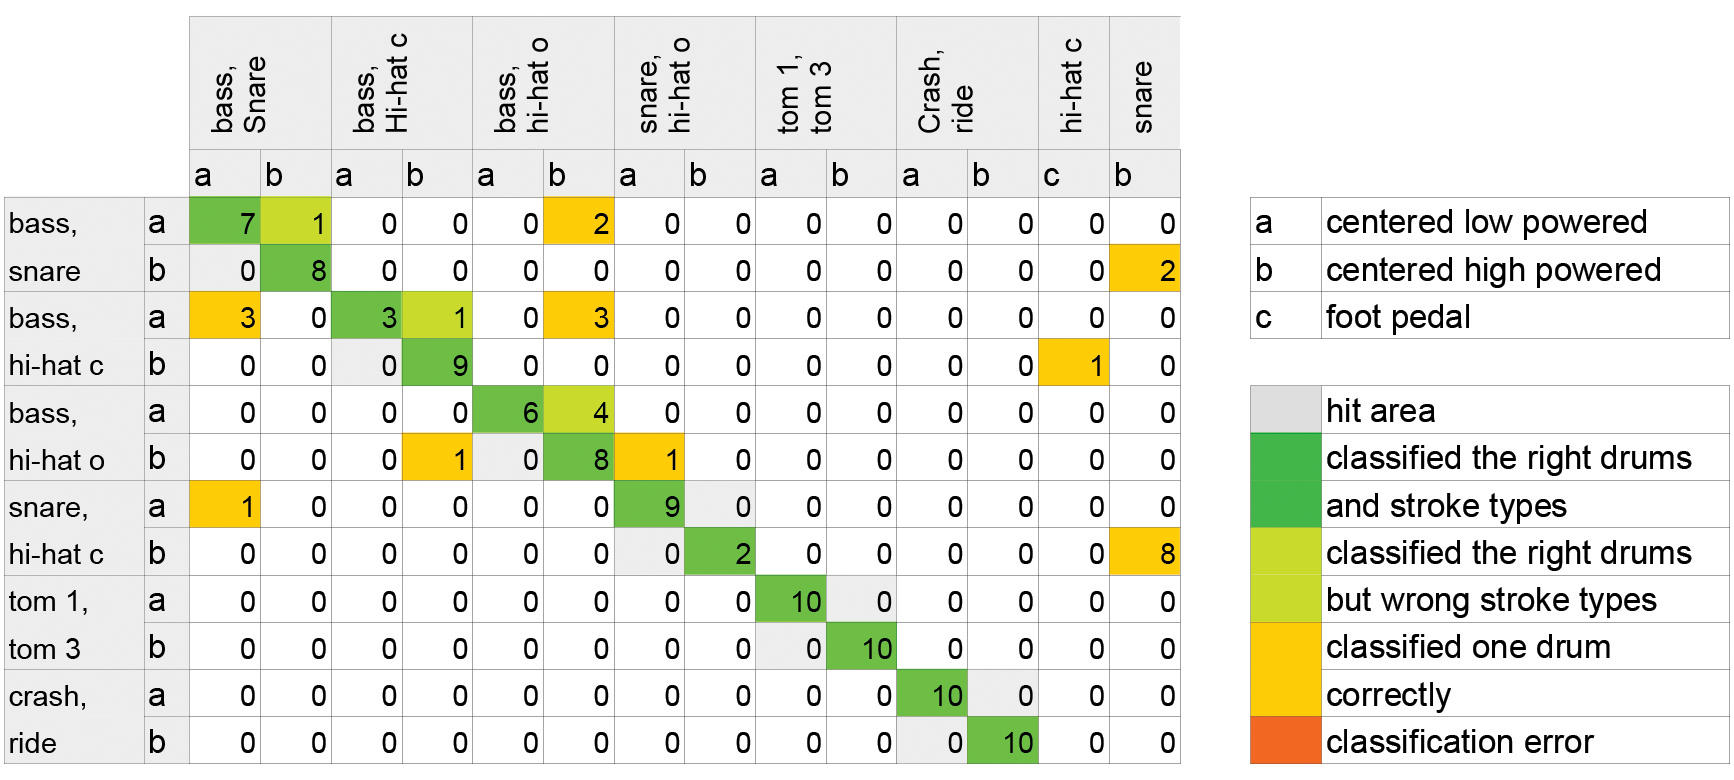
\includegraphics[width=.9\textwidth]{images/classification_matrix/multiple2_test_multiple.png}
	\caption{Results for the extended training algorithm tested with recordings containing two strokes at once.}
	\label{fig:multiple22}
\end{figure}

%\subsubsection{Comparison of classification by subtraction and classification by additional training}
%runtime!
%hitrate